\section{Embeddings}
\label{embeddings}
An embedding is a representation of a vector space that captures the similarity between the entities we are encoding, where entities can be words, images, e-commerce products, movies, houses, and many other data modalities.
Scientific progress in the field of ML is often directly about finding algorithms that can learn high-quality robust embeddings in an efficient and scalable way. The final performance of a given architecture is often largely determined by the quality of the embeddings it learns.

To illustrate this concept, we will be talking briefly about one of the earliest algorithms that has been used to learn embeddings for words: \textit{word2vec}, a technique pioneered by a team led by Thomas Mikolov.\cite{https://doi.org/10.48550/arxiv.1301.3781}
The idea behind \textit{word2vec} is to set a word into context with the words surrounding it. As it turns out, this idea that similar words appear in similar contexts, is an extremely powerful signal for achieving quality word embeddings. In NLP, the study of techniques that determine the probability of a given sequence of words is known as language modeling.

For example the word \textit{epilepsy} may appear in the context of words like \textit{symptom}, \textit{medication}, or \textit{episode} and vice versa.
However, we would not expect that \textit{epilepsy} would appear in the context of words like \textit{volleyball}.

We then translate this idea into a training task:
Given the sum of the one-hot encoded word vectors of the words surrounding the target word, map it to the one-hot encoded vector of the target word.

This is a task that can be solved by a neural network with the following setup:
Add a layer $l_1$ that maps from the input dimension (of size $|V|$) to an intermediate dimension of size $h$ and then another layer $l_2$ that maps from the intermediate dimension to the output dimension (of size $|V|$).
Here $h$ is what is called embedding dimension and $h << |V|$.

\begin{figure}
  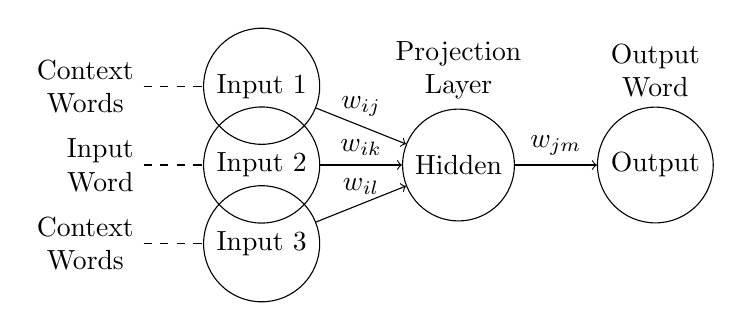
\begin{tikzpicture}[scale=1]
    % Nodes
    \node[circle, draw] (input1) at (0, 1) {Input 1};
    \node[circle, draw] (input2) at (0, 0) {Input 2};
    \node[circle, draw] (input3) at (0, -1) {Input 3};
    \node[circle, draw] (hidden) at (2.5, 0) {Hidden};
    \node[circle, draw] (output) at (5, 0) {Output};
    
    % Arrows
    \draw[->] (input1) -- (hidden) node[midway, above] {$w_{ij}$};
    \draw[->] (input2) -- (hidden) node[midway, above] {$w_{ik}$};
    \draw[->] (input3) -- (hidden) node[midway, above] {$w_{il}$};
    \draw[->] (hidden) -- (output) node[midway, above] {$w_{jm}$};
    
    % Labels
    \node[align=center, above] at (hidden.north) {Projection\\Layer};
    \node[align=center, above] at (output.north) {Output\\Word};
    
    % Input
    \draw[dashed] (-1.5, 1) -- (input1);
    \draw[dashed] (-1.5, 0) -- (input2);
    \draw[dashed] (-1.5, -1) -- (input3);
    \node[align=center, left] at (-1.5, 1) {Context\\Words};
    \node[align=center, left] at (-1.5, 0) {Input\\Word};
    \node[align=center, left] at (-1.5, -1) {Context\\Words};
    
  \end{tikzpicture}
  \caption{Illustration of the Continuous Bag of Words (CBOW) approach to the word2vec model. The model takes a window of surrounding (context) words as input, and the goal is to predict the input word. The context words are first projected onto a hidden layer, and the input word is predicted based on the activations in the hidden layer. The weights are learned through training.}
  \label{fig:word2vec_cbow}
\end{figure}

While $h$ is generally a hyperparameter that can be optimized at a later stage, a reasonable choice is to use a value according to the rule of thumb:
\begin{equation}
  h \approx 4\sqrt[\leftroot{3} \uproot{3} 4]{|V|}
\end{equation}
For a vocabulary size $|V| = 30000$ this comes to a value of about $50$.
During training, the network will learn to encode the original sparse indicator vectors in a way that preserves the maximum amount of information necessary to predict the target word, while being forced to squeeze the information through the low dimensional bottleneck.
An interesting side effect of this approach is that we can use part of the network to encode a given word in $V$ by using for example the inverse of $l_2$ as a lookup table.
The vectors that we obtain from this lookup table are called word embeddings and they have some very useful properties:
\begin{itemize}
    \item Similar words tend to be close together (e.g. in terms of Euclidean distance).
    \item Averaging word embeddings of a sentence will give us a more robust representation than our naive approach.
    \item We can perform some arithmetic, such as adding and subtracting the embedding vectors to traverse the space.
\end{itemize}
\begin{figure}
  \begin{tikzpicture}[->,>=stealth',shorten >=1pt,auto,node distance=2.8cm,
    thick,main node/.style={font=\sffamily\Large\bfseries}]

\node[main node] (w_man) at (0,0) {};
\node[above = 0mm of w_man] {$\boldsymbol{w_{\text{man}}}$};
\node[main node] (w_king) at (4,2) {};
\node[right = 0mm of w_king] {$\boldsymbol{w_{\text{king}}}$};
\node[main node] (w_woman) at (2,-2) {};
\node[below = 0mm of w_woman] {$\boldsymbol{w_{\text{woman}}}$};
\node[main node] (w_queen) at (6,0) {};
\node[right = 0mm of w_queen] {$\boldsymbol{w_{\text{queen}}}$};

\path[every node/.style={font=\sffamily\small}]
(w_man) edge[red] node [above = 3mm] {$\boldsymbol{w_{\text{king}}} - \boldsymbol{w_{\text{man}}}$} (w_king)
(w_man) edge[blue] node [below left] {$\boldsymbol{w_{\text{woman}}} - \boldsymbol{w_{\text{man}}}$} (w_woman)
(w_woman) edge[red] node [above right] {} (w_queen)
(w_king) edge[blue] node [above right] {} (w_queen);

\node[right=14mm of w_queen, font=\sffamily\small, align=center] {$\approx \textcolor{red}{\boldsymbol{w_{\text{king}}} - \boldsymbol{w_{\text{man}}}} + \boldsymbol{w_{\text{woman}}}$};

\end{tikzpicture}

  \caption{Geometric illustration of word2vec performing vector arithmetic using word embeddings. If we take the representation of "king", subtract away the representation of "man", and add the representation of "woman", the vector representation closest to the result in our vocabulary table is the vector of the word "queen".}
  \label{fig:kingmanwoman}
\end{figure}
These properties also imply that the representions for two sentences will be close together if they are semantically similar, which will make the job of, say, a downstream classifier much more straightforward - it only has to slice the embedding space.
The hard part of understanding the meaning of the sentence is already done.
Since the training data can be generated from just raw text, it is sufficient to train the embeddings once on a very large corpus and then reuse them, in effect giving us a headstart when building task-specific models.\cite{pennington-etal-2014-glove}
Instead of also having to learn what words mean, and some of the syntactic rules behind written language, we can get a head start on this and focus our computational resources on adapting this knowledge to a specific task.

Using these pre-trained text representations is often critical. Without doing so, the majority of what a machine learns is the basic syntax and semantics of language. By using these pre-trained word embeddings, we allow our models to learn to focus more on the downstream task. By simplifying the learning task with these pre-trained embeddings, we need to use far fewer labeled examples than we would training from scratch.

This underlying assumption that similar neighboring words share a semantic similarity to center words is powerful, and at the heart of many modern training objectives for embeddings that are used in many downstream ML systems.
We do not inherently inject a great deal of model bias, but rather rely on having a large enough training set that the word vectors will become meaningful representations with respect to one another.
A corpus such as Common Crawl\footnote{Common Crawl Link}, which contains roughly 840 billion tokens of over two million unique words, provides such scale.
There are other corpora used in these unsupervised processes, one such common candidate being a collection of all Wikipedia articles.

In practice, one training objective can be to use the distributed representation of a set of context words to guess a center word. This is known as the continuous bag of words (CBOW) model and is illustrated in Figure \ref{fig:word2vec_cbow}

Consider a training document describing patients with epilepsy, where we are attempting to train a model with a predefined vocabulary $V$ of the top For a vocabulary $V$, where we have chosen the top $|V|$ most common words in English to learn.
The document being chosen in this training iteration may contain the following excerpt:

\begin{verbatim}
  ... recommended administering Lamictal to treat their
  focal seizures, the patient continued experiencing
  symptoms though reported a 50% reduction in ...
\end{verbatim}

In training our word embeddings, we will randomly mask one of the words, in this case \textit{patient}.
Our model makes use of an additional parameter, a context window size $c$, that helps to provide necessary context.
If we choose $c = 8$, our training sample would become

\begin{verbatim}
  ... lamictal to treat their focal seizures, the [MASK]
  continued experiencing symptoms though reported a 50 % ...
  \end{verbatim}

For a given center word at index $i$, we consider previous words at indexes $i-1$, $i-2$, ..., $i-c$, and all subsequent words at indexes $i+1$, $i+2$, ..., $i+c$.
In our word sequence $S$, we may then choose to sum the word vectors of each of these context words.
Our context input can be written as:
\begin{equation}
  \sum_{ \substack {j=-c \\ j \neq 0}}^c w_{i+j}
\end{equation}

Our task is then to predict a probability distribution over the size of our vocabulary $|V|$, where the target is a vector of all 0's with a 1 at the index in the vocabulary for the word \textit{patient}.

There are a few additional takeaways from this example.
Note that we will address many of these in the sections to follow.
\begin{itemize}
  \item The training process will likely consider this text many times, and mask out different words in each iteration.
  \item Our processed sentence is slightly modified from our original input.
  Notice that the number and percent symbol are split, and that Lamictal is lowercased.
  \item The word \textit{patient} can also be an adjective.
  Our \textit{patient} embedding will also capture this meaning in our model, dependent upon how often it is used with that meaning.
  \item If our context window is too small, we lose information.
  If it is too large, our signal becomes fuzzy as we converge to the global mean vector.
\end{itemize}

What if we choose to use only a center word, and have our model predict all of the surrounding context words?
This is a common training technique for embeddings as well, and is known as the Skip-Gram model.

\subsection{Spacy Example of Word Embeddings}

\begin{python}
  # Example 2 - Spacy Word Embeddings
  import spacy

  sample_words = ["epilepsy", "seizure",
                  "patient", "language"]

  nlp = spacy.load("en_core_web_md")
  docs = [nlp(sample) for sample in sample_words]

  #Spacy's Medium English Model Stores Words As
  # Vectors of Dimension 300
  #Note each word has this vector size
  for doc in docs:
      assert doc.vector.shape[0] == 300

  #The cosine distance, ranging from [0,1], of
  # the vectors tells us how similar the words are
  print(docs[0].similarity(docs[1]))
  #epilepsy and seizure -> 0.9999
  print(docs[0].similarity(docs[2]))
  #epilepsy and patient -> 0.4434
  print(docs[0].similarity(docs[3]))
  #epilepsy and language -> 0.1273
\end{python}

\subsection{Character and Subword Embeddings}

In Example 1, we covered the issue of missing vocabulary that is frequently encountered when using word-level tokenization.
However, there are other strategies that are commonly used that help to avoid this issue.
One such simple way around out-of-vocabulary tokens is to use character-level tokenization.
Instead of having a vocabulary that is tens of thousands of words long, you only have a vocabulary that contains the characters in
your language, with the addition of punctuation, digits, and a few special tokens for sentence and word marking.
As long as the tokenizer is able to mark which characters start a word and which characters are continuations of a word, then the original sequence of words can always be recovered.

Unfortunately, the tradeoff for a small vocabulary size with no unknown word entries is that the length of tokens to represent a sentence is clearly much larger.
Empirically, these models do not perform as well, partially because of this sequence length but also because of the loss of information that is represented in word vectors.

In practice, the best models are often somewhere in the middle, in what is known as word-piece, or subword, vocabularies.
These tokenizers and vocabularies contain a rich set of common words, but also have subword units that can be used to piece together out-of-vocabulary words.
These subword units behave like normal word vectors and can store semantic and syntactic information.


\begin{python}
  # Example 3 - Wordpiece Tokenizers

  from transformers import BertTokenizer

  sample = "After a temporal lobe resection, the " \
           "atonic and clonic seizure frequency " \
           "fell by 50%."

  bert_tokenizer = BertTokenizer.from_pretrained(
      'bert-base-uncased'
  )

  ids = bert_tokenizer.encode(sample)
  tokens = bert_tokenizer.convert_ids_to_tokens(
      encoded_ids
  )

  for token, id  in zip(tokens, ids):
      print("{}: {}".format(token,id))

  #output:
  # [CLS] 101
  # after: 2044
  # a: 1037
  # temporal: 15850
  # lobe: 21833
  # res: 24501
  # ##ection: 18491
  # ... (output continues)
  #   %: 1003
  # .: 1012
  # [SEP]: 102
\end{python}

In the tokenizer output in example 3 above, note the following:
\begin{enumerate}
  \item The text is silently preprocessed to be lowercased. Other functions, such as whitespace trimming, are common.
  \item The output token sequence includes the specialized tokens (CLS), and (SEP), that not only help to mark the beginning and end of a sequence but aid in downstream classification in the model.
  \item The word resection is split into two tokens, with a special marker for the continuation of a word that was split.
\end{enumerate}

\subsection{Domain-Specific Medical Embeddings} \label{Domain-Specific Medical Embeddings}

Many of the datasets and models that are available online are trained on general text, and not specific to any particular domain.
Unsurprisingly, vocabularies that include medical terminology are used in practice, as are the models that have been trained to
represent these vectors in NLP tasks specific to medicine. Using these models is a common practice and often gives a better result
than a general-purpose approach. Because data collection is an expensive process, the better pre-trained embeddings we have, the
faster we can get to a high-quality model for our specialized task.

Predictive models from electronic health records have been used to train transformer-based models, and \texttt{Med-Bert}\cite{rasmy2020medbert}
is an example of one such model giving a boost to prediction accuracy with respect to the number of training examples required by a
specialized model. The \texttt{BioBERT}\cite{DBLP:journals/corr/abs-1901-08746} model,  \texttt{Bio\textunderscore ClinicalBERT}\cite{https://doi.org/10.48550/arxiv.1904.03323} model,
can be loaded as a drop-in replacement for a BERT model from the Huggingface library to achieve better results in clinical tasks. Many other such models
exist and it is recommended to keep an eye out for advancements in this respect when attempting to use pre-trained models for tasks
in not only epilepsy but other domains.
